% main.tex
\documentclass[11pt,a4paper]{article}

% ---- Language / Font ----
\usepackage[T1]{fontenc}
\usepackage[utf8]{inputenc}
\usepackage{kotex}

% ---- Layout ----
\usepackage[margin=1in]{geometry}
\usepackage{graphicx}
\graphicspath{{../../figures/}}

% ---- Math / Tables ----
\usepackage{amsmath,amssymb}
\usepackage{booktabs}
\usepackage{array}
\usepackage{longtable}

% ---- Lists / Links ----
\usepackage{enumitem}
\usepackage[hidelinks]{hyperref}

% ---- Bibliography ----
\usepackage[numbers]{natbib}

\title{Trust-Aware Backpressure RPL for Resilient Routing in LLNs under Routing Attacks}
\author{이건형}
\date{}

\begin{document}
\maketitle

\begin{abstract}
Low-Power and Lossy Networks (LLNs) rely on RPL and its backpressure-based variant BRPL to achieve stable routing under lossy links and congestion. However, these protocols do not explicitly account for insider routing attacks that manipulate data-plane forwarding or control-plane advertisements, which can lead to abrupt performance collapse beyond a topology-dependent attack intensity. This paper presents \emph{Trust-Aware BRPL}, a lightweight integration of trust-derived penalties into BRPL’s routing decision. We model data-plane reliability via a Beta-based estimator with EWMA smoothing and capture control-plane anomalies using rank-inconsistency and stability signals. Using Contiki-NG/Cooja, we conduct reproducible parameter sweeps over attack intensity, topology classes, and network scale, and compare BRPL vs. Trust-Aware BRPL in terms of packet delivery ratio (PDR), end-to-end delay, control overhead, and parent churn. The results (to be inserted) are organized to quantify how trust parameters shift the collapse threshold and to characterize the resulting resilience–overhead trade-off.
\end{abstract}

\noindent\textbf{Keywords:} RPL, BRPL, Backpressure, Trust, LLN, IoT Security, Selective Forwarding, Sinkhole, Contiki-NG, Cooja

\section{Introduction}
\label{sec:intro}
LLNs are widely used in IoT sensing and control where devices operate under strict power and memory constraints and communicate over lossy wireless links. RPL provides a standardized IPv6 routing framework for LLNs based on DODAG formation, rank, and parent selection \citep{rfc6550}. BRPL extends RPL with backpressure-inspired decisions to improve throughput and latency in the presence of congestion by exploiting path diversity \citep{moeller2016brpl}.

Despite these advances, routing in LLNs remains vulnerable to insider attacks. Two representative threats are (i) \emph{selective forwarding} (grayhole/blackhole), where a compromised forwarder probabilistically drops packets, and (ii) \emph{sinkhole} behavior, where a node attracts traffic through misleading control-plane advertisements (e.g., rank manipulation) and subsequently disrupts delivery \citep{karlof2003secure,wood2002dos,le2013rank,mayzaud2016taxonomy}. Empirically, such attacks often induce a \emph{phase-transition-like} behavior: performance degradation is small for low attack intensity but collapses sharply beyond a threshold that depends on topology and routing structure.

\subsection{Goal and Approach}
\label{subsec:goal}
This work aims to delay or mitigate this collapse by incorporating lightweight trust signals into BRPL’s decision process. Instead of introducing heavy cryptographic mechanisms or standalone intrusion detection, we integrate trust as a \emph{penalty} in the routing metric: suspected nodes become less attractive as forwarders/parents while preserving BRPL’s congestion-aware benefits.

\subsection{Contributions}
\label{subsec:contrib}
\begin{itemize}[leftmargin=*]
  \item \textbf{Trust-Aware BRPL design:} a lightweight trust-penalized BRPL metric that down-weights untrustworthy neighbors while retaining backpressure-based adaptivity.
  \item \textbf{Dual-plane trust modeling:} data-plane trust via Beta estimation with EWMA smoothing and control-plane trust via rank-inconsistency and stability signals derived from RPL semantics.
  \item \textbf{Reproducible evaluation framework:} Contiki-NG/Cooja implementation with scripted sweeps across topology classes, scales (S/M/L), and attack intensities for selective forwarding, sinkhole, and combined attacks.
  \item \textbf{Collapse-threshold analysis:} result organization that quantifies how trust parameters shift the collapse point and how resilience trades off against overhead and churn.
\end{itemize}

\subsection{Paper Organization}
Section~\ref{sec:background} reviews background and related work.
Section~\ref{sec:model} defines the system and threat model.
Section~\ref{sec:design} presents Trust-Aware BRPL.
Section~\ref{sec:impl} describes implementation.
Section~\ref{sec:setup} details experimental setup.
Section~\ref{sec:results} and Section~\ref{sec:discussion} report and discuss results.
Section~\ref{sec:conclusion} concludes.

\section{Background and Related Work}
\label{sec:background}
\subsection{RPL and BRPL}
RPL constructs a DODAG rooted at a sink and uses rank to enforce loop avoidance and convergence \citep{rfc6550}. BRPL augments RPL with backpressure principles, combining queue differentials with routing costs to improve throughput and delay under congestion, leveraging multiple paths when available \citep{moeller2016brpl}.

\subsection{Routing Attacks in LLNs}
Selective forwarding and sinkhole/rank attacks are well-studied threats that can severely degrade delivery and stability in LLNs \citep{karlof2003secure,wood2002dos,le2013rank,mayzaud2016taxonomy}. Sinkhole behavior often manifests through misleading control-plane information that attracts traffic; once positioned on critical paths, an attacker can amplify disruption.

\subsection{Trust-Based Routing}
Trust-based routing introduces behavioral reliability into routing decisions, commonly via direct observation and/or reputation systems \citep{ganeriwal2004reputation,ganeriwal2008tosn,momani2010survey}. In LLNs, imperfect wireless observations and limited overhearing motivate lightweight estimators and smoothing rather than full watchdog schemes.

\section{System and Threat Model}
\label{sec:model}
\subsection{System Model}
We use Contiki-NG and Cooja to simulate 6LoWPAN/IPv6 LLN stacks with RPL/BRPL routing. Traffic follows a many-to-one periodic pattern from sensor nodes to a root. Nodes maintain neighbor tables and select preferred parents according to the underlying routing logic \citep{rfc6550,moeller2016brpl}.

\subsection{Threat Model}
We consider a single insider attacker (extensions to multiple attackers are future work). The attacker participates as a normal node but executes one of the following:
\begin{itemize}[leftmargin=*]
  \item \textbf{Selective forwarding:} probabilistic packet dropping on forwarded traffic, with drop probability swept as attack intensity.
  \item \textbf{Sinkhole (rank manipulation):} control-plane manipulation to attract traffic (e.g., advertising an artificially low rank), followed by normal forwarding unless combined with dropping.
  \item \textbf{Combined attack:} sinkhole attraction plus selective forwarding on captured flows.
\end{itemize}
We assume the root is non-malicious. Cryptographic authentication and secure bootstrapping are outside the scope of this paper.

\section{Trust-Aware BRPL Design}
\label{sec:design}
This section defines trust signals and how they modulate BRPL decisions. We denote by $i$ the observing node and $j$ a neighbor candidate (potential parent/forwarder). Trust values are normalized to $[0,1]$ where larger is better.

\subsection{Data-Plane Trust for Selective Forwarding}
\label{subsec:grayhole}
We model forwarding reliability as the probability that a neighbor forwards packets successfully. Let $s_j$ and $f_j$ denote observed successful and failed forwarding events attributed to $j$ (e.g., via log-based inference). Using a Beta prior $(\alpha_0,\beta_0)$ for Bernoulli forwarding outcomes \citep{ganeriwal2004reputation,ganeriwal2008tosn}, the posterior mean is
\begin{equation}
\hat{T}_{\text{gray}}(j)=\frac{\alpha_0+s_j}{\alpha_0+\beta_0+s_j+f_j}.
\end{equation}
To reduce short-term noise, we apply EWMA smoothing:
\begin{equation}
T_{\text{gray}}(j;t)=\rho\,T_{\text{gray}}(j;t\!-\!1)+(1-\rho)\,\hat{T}_{\text{gray}}(j),
\end{equation}
where $\rho\in[0,1)$ controls smoothing.

\subsection{Control-Plane Trust for Sinkhole Behavior}
\label{subsec:sinkhole}
Sinkhole attacks primarily affect control-plane advertisements. RPL rank semantics impose monotonicity constraints on feasible parent relations \citep{rfc6550}. Let $R_i$ be node $i$’s current rank and $R_j$ the advertised rank from neighbor $j$. Define
\begin{equation}
\Delta_{ij}=R_j+\mathrm{MIN\_HOPRANKINC}-R_i.
\end{equation}
If $j$ advertises an implausibly low rank relative to $i$, $\Delta_{ij}$ becomes negative. We define a deviation score with tolerance $\tau\ge 0$:
\begin{equation}
s_{ij}=\max(0,\,-\Delta_{ij}-\tau),
\end{equation}
and map it to an exponential trust decay \citep{sun2005trust,chen2010trust}:
\begin{equation}
T_{\text{adv}}(j)=\exp(-\lambda_{\text{adv}}\,s_{ij}),
\end{equation}
where $\lambda_{\text{adv}}>0$ sets sensitivity.

Sinkhole behavior can also induce instability in rank evolution and parent selection. Over a window $W$, define rank increase
\begin{equation}
\Delta R_i=R_i(t)-R_i(t-W),
\end{equation}
and penalize abnormal increases beyond $\kappa\ge 0$:
\begin{equation}
u_i=\max(0,\,\Delta R_i-\kappa), \qquad
T_{\text{stab}}(t)=\exp(-\lambda_{\text{stab}}\,u_i).
\end{equation}
We combine control-plane signals multiplicatively:
\begin{equation}
T_{\text{sink}}(j)=\left(T_{\text{adv}}(j)\right)^{w_1}\left(T_{\text{stab}}(t)\right)^{w_2},
\end{equation}
with weights $w_1,w_2\ge 0$.

\subsection{Total Trust Aggregation}
\label{subsec:totaltrust}
We aggregate data-plane and control-plane trust via a weighted geometric mean:
\begin{equation}
T_{\text{total}}(j)=\left(T_{\text{gray}}(j)\right)^{\alpha}\left(T_{\text{sink}}(j)\right)^{1-\alpha},
\end{equation}
where $\alpha\in[0,1]$ controls the emphasis on selective-forwarding vs. sinkhole signals.

\subsection{Trust-Penalized BRPL Metric}
\label{subsec:metric}
Let $BP_{ij}$ denote the baseline BRPL weight/utility for neighbor $j$ from node $i$ (as defined by BRPL’s backpressure and cost combination) \citep{moeller2016brpl}. We define a trust penalty factor
\begin{equation}
\phi(T)=\frac{T^{\gamma}}{1+\lambda\,(1-T)^{\gamma}},
\label{eq:phi}
\end{equation}
where $\lambda\ge 0$ controls avoidance aggressiveness and $\gamma\ge 1$ controls risk sensitivity. The trust-aware metric is
\begin{equation}
BP^{\text{(trust)}}_{ij}=BP_{ij}\cdot \phi\!\left(T_{\text{total}}(j)\right).
\end{equation}
This form preserves ordering when trust is uniform, while strongly down-weighting neighbors with low trust as $\lambda$ or $\gamma$ increases. The use of tunable penalty parameters follows common drift-plus-penalty / risk-sensitive control intuition in stochastic network optimization \citep{neely2010}.

\subsection{Algorithm Outline}
\label{subsec:algo}
At each decision epoch, node $i$:
\begin{enumerate}[leftmargin=*]
  \item Updates trust values (data-plane and/or control-plane) and clamps to $[0,1]$.
  \item For each neighbor candidate $j$, computes $BP^{\text{(trust)}}_{ij}$.
  \item Selects the preferred parent / forwarding next hop that maximizes the trust-penalized objective, with optional hysteresis to reduce churn.
\end{enumerate}

\subsection{Overhead}
\label{subsec:overhead}
Trust maintenance stores $O(\deg)$ values per node, where $\deg$ is neighbor degree. The metric adds $O(\deg)$ arithmetic per decision. No additional control packets are required by design; any extra overhead arises from changed routing dynamics (e.g., parent switching).

\section{Implementation in Contiki-NG}
\label{sec:impl}
We implement Trust-Aware BRPL in Contiki-NG by integrating the trust penalty into the BRPL metric computation and parent selection path. The attacker node supports:
(i) probabilistic forwarding drops for selective forwarding,
(ii) rank advertisement manipulation for sinkhole behavior, and
(iii) combined operation.

All trust values used for routing decisions are computed and applied \emph{online} during the simulation runtime, while the trust engine additionally performs \emph{offline} log-based analysis solely for measurement, visualization, and reproducibility purposes; offline results are never fed back into routing decisions.

To support measurement and reproducibility, we maintain a scripted pipeline that runs batch experiments over seeds, topologies, and attack parameters, and extracts metrics from Cooja logs. Implementation-specific file names and scripts are omitted from the main narrative and can be provided as an artifact alongside the code repository.

\begin{figure}[t]
  \centering
  \includegraphics[width=0.9\linewidth]{architecture.pdf}
  \caption{Software architecture of Trust-Aware BRPL and its integration into the Contiki-NG protocol stack.}
  \label{fig:arch}
\end{figure}

\begin{figure}[t]
  \centering
  \includegraphics[width=0.9\linewidth]{trust_update_flow.pdf}
  \caption{Online trust update and routing decision flow executed at each node during simulation runtime.}
  \label{fig:trust-flow}
\end{figure}

\section{Experimental Setup}
\label{sec:setup}
\subsection{Simulation Environment}
We use the UDGM Distance Loss radio model in Cooja \citep{osterlind2006cooja}. Unless otherwise stated, simulations run for 600\,s with a 120\,s warm-up. Sensor nodes generate periodic traffic to the root every 30\,s. RPL Trickle parameters follow a standard configuration derived from RPL’s design trade-offs between stability and control overhead \citep{rfc6550}.

\subsection{Topologies and Scales}
We evaluate multiple topology \emph{classes} to cover different path diversity regimes:
\begin{itemize}[leftmargin=*]
  \item \textbf{Grid:} high path diversity; attacks may be partially bypassed.
  \item \textbf{Two-cluster with bottleneck:} a constrained cut; attacks are amplified when the attacker sits near the bottleneck.
  \item \textbf{Corridor/chain:} low path diversity; collapse can occur at lower intensities.
  \item \textbf{Ring/spokes:} intermediate diversity; highlights root-near and mid-path influence.
\end{itemize}
We scale network size as S/M/L (e.g., 16/36/64 nodes including the root) while preserving the same placement rule per class. Attacker placement follows a rule-based selection (e.g., central relay candidate or bottleneck vicinity) to avoid ad-hoc tuning.

\begin{figure}[p]
  \centering
  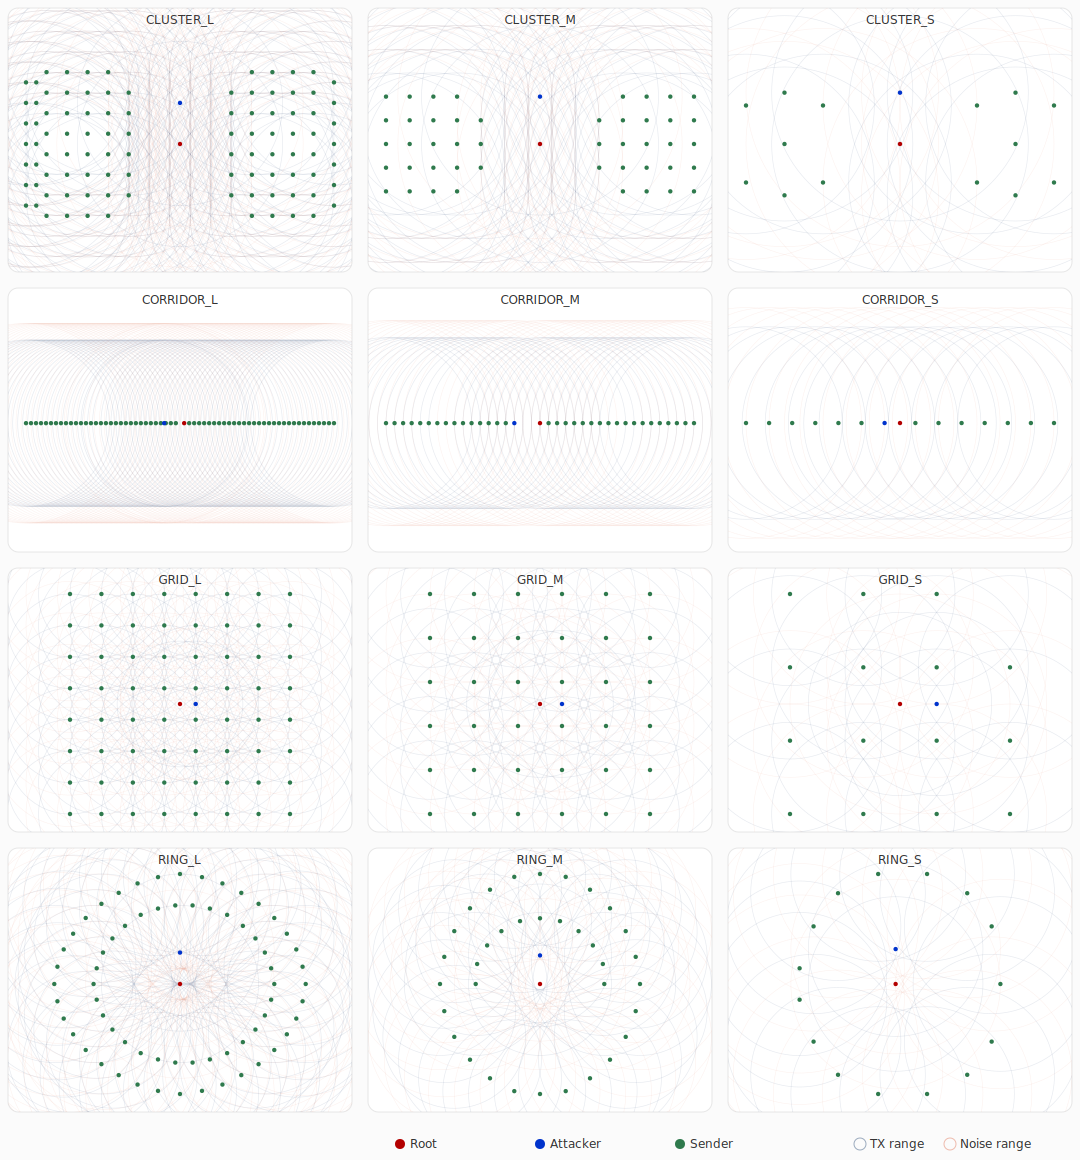
\includegraphics[width=\textwidth,height=\textheight,keepaspectratio]{topology_svgs/all_topologies.pdf}
  \caption{Topology layouts used for evaluation, covering different path diversity regimes and attacker positions.}
  \label{fig:all-topologies}
\end{figure}

\subsection{Attack Configuration}
Selective forwarding is parameterized by drop probability (e.g., 0/30/50/70\%). Sinkhole intensity is parameterized by a rank manipulation delta (e.g., 1/2/4). We evaluate three modes: selective forwarding only, sinkhole only, and combined.

\begin{figure}[t]
  \centering
  \includegraphics[width=0.9\linewidth]{experiment_workflow.pdf}
  \caption{Experiment workflow from simulation execution to offline metric extraction.}
  \label{fig:workflow}
\end{figure}

\subsection{Trust Model Parameters}
\label{subsec:trust-params}

Table~\ref{tab:trust-params} summarizes the trust-related parameters used throughout the experiments. Unless otherwise stated, the same configuration is applied across all topologies and scales to avoid per-scenario tuning.

\begin{table}[t]
\centering
\caption{Trust model parameters used in experiments.}
\label{tab:trust-params}
\begin{tabular}{lll}
\toprule
Parameter & Description & Value \\
\midrule
$\alpha_0$ & Beta prior (success) & 1 \\
$\beta_0$  & Beta prior (failure) & 1 \\
$\rho$     & EWMA smoothing factor & 0.8 \\
$W$        & Rank stability window & 5 sampling intervals \\
$\tau$     & Rank deviation tolerance & 0 \\
$\kappa$   & Rank increase tolerance & 0 \\
$\lambda_{\text{adv}}$ & Rank anomaly sensitivity & 0.01 \\
$\lambda_{\text{stab}}$ & Rank instability sensitivity & 0.01 \\
$w_1$      & Weight of rank inconsistency trust & 0.5 \\
$w_2$      & Weight of rank stability trust & 0.5 \\
$\alpha$   & Grayhole vs. sinkhole trust weight & \{1.0, 0.5\} \\
$\lambda$  & Trust penalty strength & \{0, 1, 3, 10\} \\
$\gamma$   & Risk sensitivity exponent & \{1, 2, 4\} \\
\bottomrule
\end{tabular}
\end{table}

\subsection{Metrics}
We report:
\begin{itemize}[leftmargin=*]
  \item \textbf{PDR:} $\mathrm{RX}_{\text{root}} / \mathrm{TX}_{\text{senders}}$.
  \item \textbf{End-to-end delay:} per-packet latency from source to root.
  \item \textbf{Control overhead:} control-plane transmissions (e.g., DIO/DAO) and routing-related overhead.
  \item \textbf{Parent churn:} parent switching rate, reflecting routing stability.
  \item \textbf{Exposure (optional):} fraction of delivered packets traversing the attacker and/or fraction of time the attacker is a preferred parent (used to interpret attack effectiveness).
\end{itemize}

\subsection{Parameter Sweeps}
We sweep:
(i) attack intensity,
(ii) topology class and scale,
(iii) trust aggregation weight $\alpha$,
(iv) penalty parameters $(\lambda,\gamma)$ for trust-aware cases.
Multiple random seeds are used to report mean and variability.

\begin{table}[t]
\centering
\caption{Core experimental parameters (default).}
\label{tab:params}
\begin{tabular}{ll}
\toprule
Parameter & Value \\
\midrule
Field size & 200 m $\times$ 200 m \\
Radio model & UDGM Distance Loss \\
TX range / Interference range & 45 m / 90 m \\
Simulation time / Warm-up & 600 s / 120 s \\
Traffic interval & 30 s \\
Root ID & 1 \\
Attacker count & 1 (default) \\
\bottomrule
\end{tabular}
\end{table}

\section{Results}
\label{sec:results}
This section will be finalized after data collection. We structure the analysis to highlight (i) collapse threshold behavior and (ii) trade-offs induced by trust penalization.

\begin{figure}[t]
  \centering
  \fbox{\parbox{0.9\linewidth}{\centering Fig.~3 (placeholder): PDR vs. attack intensity by topology/scale}}
  \caption{PDR vs. attack intensity (placeholder).}
  \label{fig:pdr}
\end{figure}

\begin{figure}[t]
  \centering
  \fbox{\parbox{0.9\linewidth}{\centering Fig.~4 (placeholder): delay vs. attack intensity}}
  \caption{End-to-end delay vs. attack intensity (placeholder).}
  \label{fig:delay}
\end{figure}

\begin{figure}[t]
  \centering
  \fbox{\parbox{0.9\linewidth}{\centering Fig.~5 (placeholder): control overhead vs. attack intensity}}
  \caption{Control overhead vs. attack intensity (placeholder).}
  \label{fig:overhead}
\end{figure}

\begin{figure}[t]
  \centering
  \fbox{\parbox{0.9\linewidth}{\centering Fig.~6 (placeholder): parent churn vs. attack intensity}}
  \caption{Parent churn vs. attack intensity (placeholder).}
  \label{fig:parent-switch}
\end{figure}

\begin{figure}[t]
  \centering
  \fbox{\parbox{0.9\linewidth}{\centering Fig.~7 (placeholder): $(\lambda,\gamma)$ sweep trade-off surface}}
  \caption{Trade-off under trust penalty sweeps (placeholder).}
  \label{fig:lambda-tradeoff}
\end{figure}

\section{Discussion}
\label{sec:discussion}
We discuss how topology-dependent path diversity and attacker placement influence collapse thresholds, and how trust penalization shifts these thresholds. We also analyze (i) potential false positives under wireless loss and transient dynamics, (ii) sensitivity to $(\lambda,\gamma,\alpha)$, and (iii) stability impacts reflected in churn and overhead. Importantly, the proposed mechanism is intended to complement—not replace—cryptographic protections and secure bootstrapping, providing resilience gains even when full authentication is unavailable or impractical.

\section{Conclusion and Future Work}
\label{sec:conclusion}
We presented Trust-Aware BRPL, which integrates lightweight trust penalties into BRPL routing decisions using both data-plane reliability and control-plane anomaly signals. The evaluation plan is designed to quantify how trust parameters delay performance collapse under selective forwarding and sinkhole attacks and to characterize the resilience–overhead trade-off across topologies and scales. Future work includes multiple colluding attackers, adaptive tuning of trust penalty parameters, and validation on real testbeds.

\bibliographystyle{plainnat}
\bibliography{references}

\end{document}
